%!TEX root = ../../../main.tex

\section{Linear-time logic}

% ---------------------------------------------------------------------

\begin{frame}{Preliminaries}

\hl{Linear-time logic} in general:
\begin{itemize}
\item any logic working with sequences of valuations
\item model: time progresses in discrete steps and in linear fashion, each point in time has exactly one possible future
\item origins in philosophy/logic
\end{itemize}

\bigskip
Most prominent species: \hl{LTL}
\begin{itemize}
\item in use for verification since end of the 1970s
\item \hl{spezification} of correctness properties
\end{itemize}
\end{frame}

% ---------------------------------------------------------------------

\begin{frame}{Recap}
\begin{itemize}
\itemsep1em
\item Let \m{AP} be a set of atomic propositions.

\item \m{2^{AP}} denotes the powerset of \m{AP},
   i.e.\ its set of subsets.

\item \m{(2^{AP})^\omega} denotes the set of
  (infinite) sequences of valuations (of \m{AP}).\\[20mm]
\end{itemize}
\end{frame}

% ---------------------------------------------------------------------

\begin{frame}{Syntax of LTL}

Let $AP$ be a set of atomic propositions. The set of \hl{LTL formulae} over $AP$ is inductively defined as follows:

\bigskip
\begin{itemize}
\itemsep1em
\item If $p\in AP$ then $p$ is a formula.

\item If $\phi_1,\phi_2$ are formulae then so are:
\item[] $\neg\phi_1, \qquad \phi_1\lor\phi_2, 
\qquad \hl{\X}\phi_1, \qquad \phi_1\hl{\U}\phi_2$
\end{itemize}

\bigskip
Intuitive meaning:
$\hl{\X}\>\widehat{=}\>$ ``next'',
$\hl{\U}\>\widehat{=}\>$ ``until''.

\end{frame}

% ---------------------------------------------------------------------

\begin{frame}{Semantics of LTL}

Let \m{\phi} be an LTL formula and \m{\sigma} a valuation sequence.\\
We write \m{\sigma\models\phi} for ``\m{\sigma} satisfies \m{\phi}.''

 \begin{center}
  \(\begin{array}[t]{rl@{\hskip2em}l}
    \sigma\models & p & \hbox{if \m{p\in AP} and $p\in \sigma(0)$} \\
    \sigma\models & \neg\phi & \hbox{if $\sigma\not\models\phi$}\\
    \sigma\models & \phi_1\lor\phi_2 & \hbox{if
  $\sigma\models\phi_1$ or $\sigma\models\phi_2$}\\
    \sigma\models & \hl{\X}\phi & \hbox{if $\sigma^1\models\phi$}\\
    \sigma\models & \phi_1\hl{\U}\phi_2 & \hbox{if \m{\exists i\colon
    \big(\sigma^i\models\phi_2
   \ \ \land \ \ \forall k<i\colon \sigma^k\models\phi_1\big)}}\\
    \end{array}\)
\end{center}

\bigskip
Semantics of \m{\phi}: \qquad
  $\sem{\phi} = \{\,\sigma\mid\sigma\models\phi\,\}$

\end{frame}

% ---------------------------------------------------------------------

\begin{frame}{Examples}

Let \m{AP=\{p,q,r\}}. Find out whether the sequence
    $$\sigma=\{p\}\ \{q\}\ \{p\}^\omega$$
 satisfies the following formulae:

\begin{center}\(\begin{array}[t]{c}
p \\
q \\
\hl{\X} q \\
\hl{\X} \neg p  \\
p \hl{\U} q  \\
q \hl{\U} p  \\
(p\lor q) \hl{\U} r 
\end{array}\)\end{center}

\end{frame}

% ---------------------------------------------------------------------

\begin{frame}{Extended syntax}
We commonly use the following abbreviations:

\bigskip\small
  \(\begin{array}[t]{rcl@{\quad}rcl}
      \phi_1\land\phi_2 & \equiv & \neg(\neg\phi_1\lor\neg\phi_2) &
      \F\phi            & \equiv & {\bf true}\U\phi\\
      \phi_1\to\phi_2   & \equiv & \neg\phi_1\lor\phi_2 &
      \G\phi            & \equiv & \neg\F\neg\phi\\
      {\bf true}        & \equiv & a\lor\neg a &
      \phi_1\W\phi_2    & \equiv & (\phi_1\U\phi_2)\lor\G\phi_1\\
      {\bf false}       & \equiv & \neg{\bf true} &
      \phi_1\R\phi_2    & \equiv & \neg(\neg\phi_1\U\neg\phi_2)\\
    \end{array}\)

\bigskip
Meaning:
$\F\>\widehat{=}\>$ ``finally'' (eventually),\ \ 
$\G\>\widehat{=}\>$ ``globally'' (always),\\
\ \phantom{Meaning:}%
$\W\>\widehat{=}\>$ ``weak until'',\ \ 
$\R\>\widehat{=}\>$ ``release''.

\end{frame}

% ---------------------------------------------------------------------

\begin{frame}{Some example formulae}

\hl{Invariant:} $\G \neg(\mathit{cs}_1 \wedge \mathit{cs}_2)$
\begin{itemize}
  \item $cs_1$ and $cs_2$ are never true at the same time.
\end{itemize}
Remark: This particular form of invariant is also called
  \hl{mutex property} (``mutual exclusion'').

\bigskip
\hl{Safety:} $(\neg x)\W y$
\begin{itemize}
\item $x$ does not occur before y has happend.
\end{itemize}
Remark: It may happen that $y$ never happens in which case $x$
  also never happens.

\bigskip
\hl{Liveness:} $(\neg x)\hl{\U} y$
\begin{itemize}
\item $x$ does not occur before $y$
   \red{and} $y$ eventually happens.
\end{itemize}

\end{frame}

% ---------------------------------------------------------------------

\begin{frame}{More examples}

$\G\F p$
\begin{itemize}
\item $p$ occurs infinitely often.
\end{itemize}

$\F\G p$
\begin{itemize}
\item At some point $p$ will continue to hold forever.
\end{itemize}

$\G (\mathit{try_1} \rightarrow \F \mathit{cs_1})$
\begin{itemize}
\item For mutex algorithms: Whenever process~1 tries to enter its
   critical section it will eventually succeed.
\end{itemize}

\end{frame}

% ---------------------------------------------------------------------

\begin{frame}{Tautology, equivalence}
\begin{itemize}
\itemsep1em
\item Certain oncepts from propositional logic
   can be transferred to LTL.

\item \hl{Tautology}: A formula \m{\phi} with \m{\sema{\phi}=(2^{AP})^\omega}
   is called tautology.

\item \hl{Unsatisfiability}: A formula \m{\phi} with \m{\sema{\phi}=\emptyset}
   is called unsatisfiable.

\item \hl{Equivalence}: Two formulae \m{\phi_1,\phi_2} are called equivalent
    iff\ \m{\sema{\phi_1}=\sema{\phi_2}}.\\
    \ \phantom{Equivalence:}Denotation: \m{\phi_1\equiv\phi_2}
\end{itemize}
\end{frame}

% ---------------------------------------------------------------------

\begin{frame}{Equivalences: relations between operators}
$$\begin{array}{rcl}
\hl{\X} (\phi_1 \vee \phi_2) & \equiv & \hl{\X} \phi_1 \: \vee \: \hl{\X} \phi_2   \\
\hl{\X} (\phi_1 \wedge \phi_2) & \equiv & \hl{\X} \phi_1 \: \wedge \: \hl{\X} \phi_2   \\
\hl{\X} \neg \phi & \equiv & \neg \hl{\X} \phi \\[0.3cm]
\F (\phi_1 \vee \phi_2) & \equiv & \F \phi_1 \: \vee \: \F \phi_2   \\
\neg \F \phi& \equiv & \G \neg \phi \\[0.3cm]
\G (\phi_1 \wedge \phi_2)&\equiv & \G \phi_1 \: \wedge \: \G \phi_2 \\
\neg \G \phi& \equiv & \F \neg \phi \\[0.3cm]
(\phi_1 \wedge \phi_2) \hl{\U} \psi & \equiv & (\phi_1 \hl{\U} \psi) \: \wedge \: (\phi_2 \hl{\U} \psi)\\
\phi \hl{\U} (\psi_1 \vee \psi_2) & \equiv & (\phi \hl{\U} \psi_1) \: \vee \: (\phi \hl{\U} \psi_2)
\end{array}$$
\end{frame}

% ---------------------------------------------------------------------

\begin{frame}{Equivalences: idempotence and recursion laws}
$$\begin{array}{rcl}
\F \phi & \equiv & \F \F \phi    \\[0.3cm]
\G \phi & \equiv & \G \G \phi    \\[0.3cm]
\phi \hl{\U} \psi & \equiv & \phi \hl{\U} (\phi \hl{\U} \psi) \\[2cm]

\F \phi & \equiv & \phi \vee \hl{\X} \F \phi \\[0.3cm]
\G \phi & \equiv & \phi \wedge \hl{\X} \G \phi \\[0.3cm]
\phi \hl{\U} \psi & \equiv & \psi \vee (\phi \wedge \hl{\X} (\phi \hl{\U} \psi)) \\[0.3cm]
\phi \W \psi & \equiv & \psi \vee (\phi \wedge \hl{\X} (\phi \W \psi))
\end{array}$$
\end{frame}

% ---------------------------------------------------------------------

\begin{frame}{Interpretation of LTL on Kripke structures}
\begin{itemize}
\itemsep1em  
\item Let ${\cal K}=(S,\mathord{\to},r,AP,\nu)$ be a Kripke structure.\\
 We are interested in the valuation sequences generated by \m{\cal K}.

\item Let \m{\rho} in \m{S^\omega} be an infinite path of \m{\cal K}.

\item We assign to \m{\rho} an ``image'' $\nu(\rho)$
   in $(2^{AP})^\omega$; for all $i\ge0$ let
  $$\nu(\rho)(i) = \nu(\rho(i))$$
   i.e.\ $\nu(\rho)$ is the corresponding valuation sequence.

\item Let \m{\sema{\cal K}} denote the set of all such sequences:
$$\sema{\cal K} = \{\,\nu(\rho)\mid \hbox{$\rho$ is
    an infinite path of $\cal K$}\,\}$$
\end{itemize}
\end{frame}

% ---------------------------------------------------------------------

\begin{frame}{The LTL model-checking problem}
\begin{itemize}
\itemsep1em
\item\hl{Problem:} Given a Kripke structure
    ${\cal K}=(S,\mathord{\to},r,AP,\nu)$
   and an LTL formula \m{\phi} over \m{AP}, does
  \m{\sema{\cal K}\subseteq\sema{\phi}} hold?

\item\hl{Definition:} If \m{\sema{\cal K}\subseteq\sema{\phi}}
  then we write ${\cal K}\models\phi$.

\item\hl{Interpretation:} \red{Every} execution of \m{\cal K} must 
  satisfy \m{\phi} for \m{{\cal K}\models\phi} to hold.

\item\hl{Remark:} We may have ${\cal K}\not\models\phi$
   \red{and} ${\cal K}\not\models\neg\phi$!
\end{itemize}
\end{frame}

% ---------------------------------------------------------------------

\begin{frame}{Example}

Consider the following Kripke structure \m{{\cal K}} with \m{AP=\{p\}}:

\begin{center}
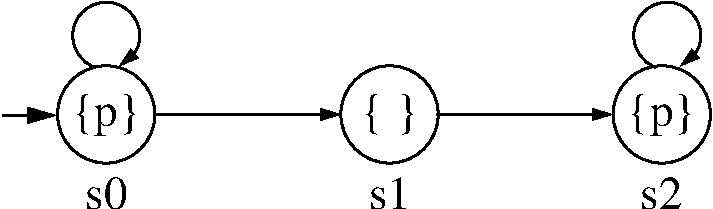
\includegraphics[scale=.4]{content/chapter_model_checking/model_checking/images/ctl-ltl}
\end{center}

\bigskip                  
There are two classes of infinite paths in \m{\cal K}:
\begin{itemize}
\item (i) Either the system stays in \m{s_0} forever,
\item (ii) or it eventually reaches \m{s_2} via \m{s_1} and remains there.
\end{itemize}

\bigskip
We have:
\begin{itemize}
\item \m{{\cal K}\models\F\G p} because all runs eventually end in a state
   satisfying \m{p}.
\item \m{{\cal K}\not\models\G p} because executions of type~(ii) contain
   a non-\m{p} state.
\end{itemize}

\end{frame}

% ---------------------------------------------------------------------

\begin{frame}{Dealing with deadlocks}

The definition of the model-checking problem only considers the
infinite sequences!

\bigskip
Thus, executions reaching a deadlock (i.e.\ a state without any
successor) will be ignored, with possibly unforeseen consequences:
\begin{itemize}
\item Suppose \m{\cal K} contains an error, so that every execution reaches
    a deadlock.
\item Then \m{\sema{\cal K}=\emptyset}, so \m{\cal K} satisfies
   \emph{every} formula, according to the definition.
\end{itemize}

\end{frame}

% ---------------------------------------------------------------------

\begin{frame}{Possible alternatives}

Remove deadlocks by design:
\begin{itemize}
\item equip deadlock states with a self loop
\item Interpretation: system stays in deadlock forever
\item adapt formula accordingly, if necessary
\end{itemize}

\bigskip
Treat deadlocks specially:
\begin{itemize}
\item Check for deadlocks before LTL model checking, deal with them separately.
\end{itemize}

\end{frame}

% ---------------------------------------------------------------------